\section{问题一：仅考虑垂荡运动的响应求解}

\subsection{二自由度垂荡模型}

\begin{figure}[H]
  \centering
  % 左图，占0.45行宽
  \begin{minipage}{0.45\textwidth}
    \centering
    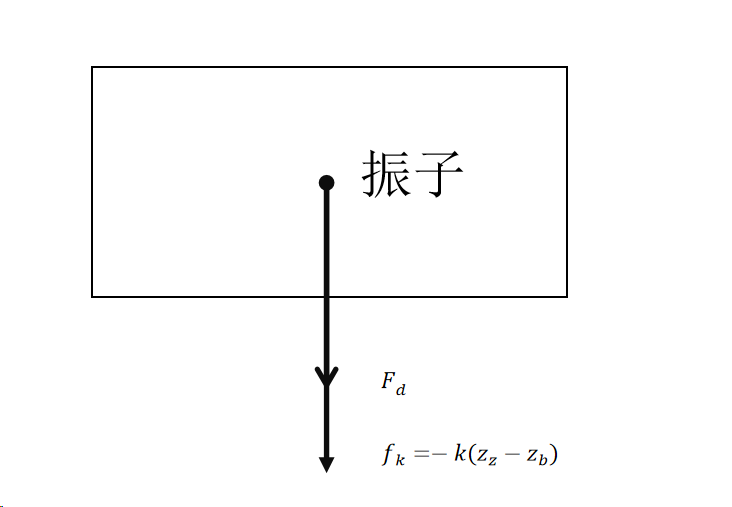
\includegraphics[width=\linewidth]{fig_problem1_model_1.png}
    \subcaption{振子}
  \end{minipage}
  % 两张图中间留间隙
  \hfill
  % 右图
  \begin{minipage}{0.45\textwidth}
    \centering
    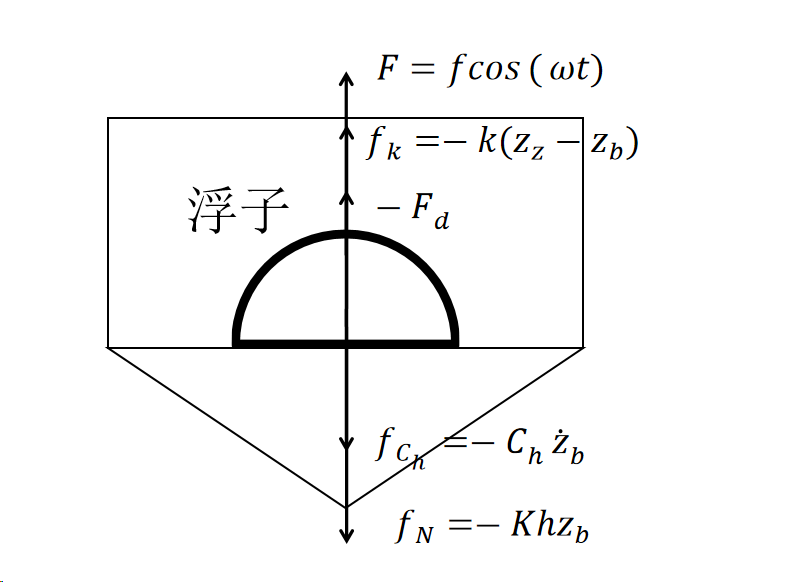
\includegraphics[width=\linewidth]{fig_problem1_model_2.png}
    \subcaption{浮子}
  \end{minipage}
  % 总图题
  \caption{系统受力分析}
  \label{fig:raw_resample}
\end{figure}

仅考虑垂荡时，取向下为正方向，浮子和振子的状态变量分别为 $z_b,z_z$。设相对位移为 $z_b-z_z$，相对速度为 $\dot z_b-\dot z_z$。线性阻尼情形下 PTO 阻尼力为
\begin{equation}
  F_d=c(\dot z_b-\dot z_z),
\end{equation}
非线性阻尼情形下阻尼系数随相对速度变化，本文采用题意对应形式
\begin{equation}
  F_d=c|\dot z_b-\dot z_z|^\alpha(\dot z_b-\dot z_z).
\end{equation}
弹簧的弹力为
\begin{equation}
  f_k=-k(z_z-z_b).
\end{equation}
令 $F_{\mathrm{PTO}}=f_k+F_d$，则浮子和振子垂荡方程为
\begin{align}
  (m_b+m_a)\ddot z_b
  &=f\cos\omega t-C_h\dot z_b-K_hz_b-F_{\mathrm{PTO}},\\
  m_z\ddot z_z&=F_{\mathrm{PTO}} .
\end{align}
初始时刻系统处于静水平衡状态，取 $z_b=z_z=\dot z_b=\dot z_z=0$。

\subsection{数值求解与结果}

将上述二阶方程化为一阶状态方程后，采用 Runge--Kutta 方法在 40 个波浪周期内积分，输出间隔为 $0.2\,\mathrm{s}$。图~\ref{fig:p1_response} 给出了线性阻尼和非线性阻尼下浮子、振子的垂荡响应。

\begin{figure}[H]
      \centering
      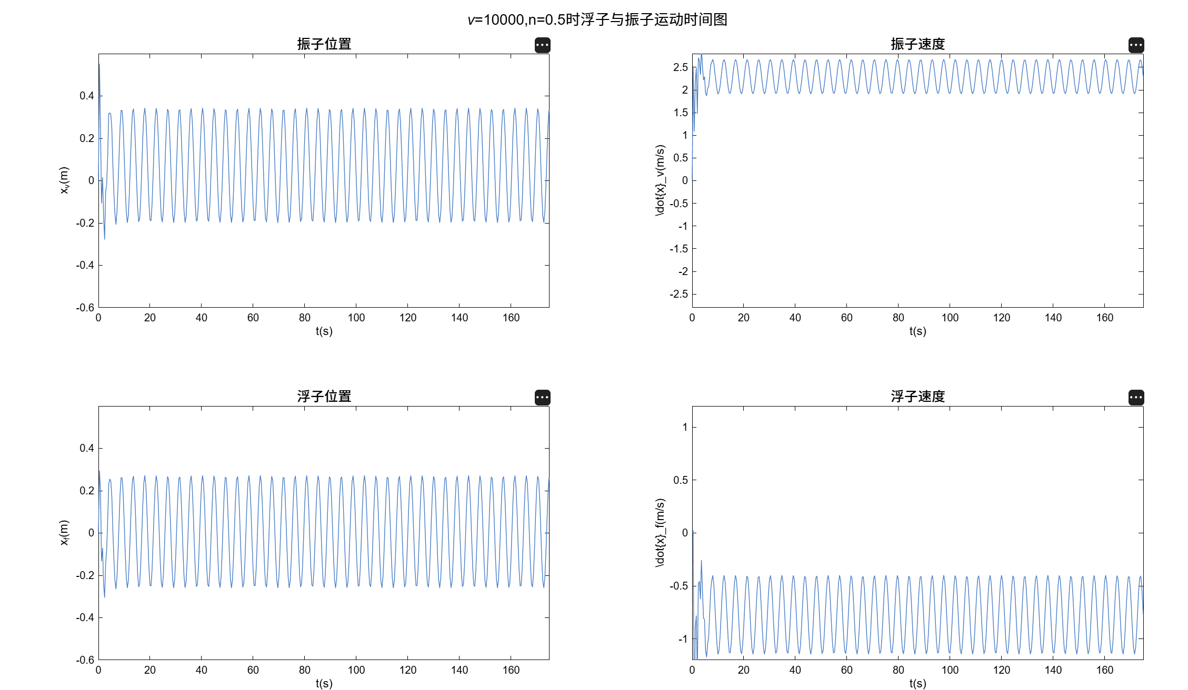
\includegraphics[width=0.75\linewidth]{fig+problem1_xiugai.png}
    \caption{问题一两种阻尼形式下的垂荡响应}
  \label{fig:p1_response}
\end{figure}

\begin{figure}[H]
    \centering
    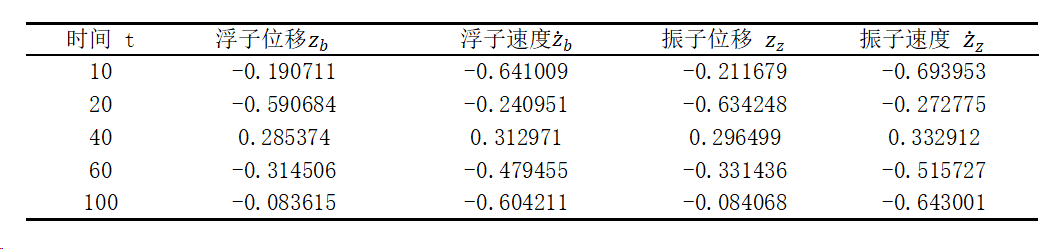
\includegraphics[width=0.75\linewidth]{fig_problem1_data.png}
    \caption{几个时间点的相关数据}
    \label{fig:placeholder3}
\end{figure}

由图可见，浮子在波浪激励下产生周期性垂荡，振子因惯性与 PTO 连接产生相位差，相对运动为阻尼器输出功率提供来源。非线性阻尼改变了相对速度较小时的阻尼强度，因此响应曲线与线性阻尼略有差异，但整体仍表现为受迫振动并逐渐进入稳定周期运动。
